\documentclass[11pt]{article}
\usepackage[a4paper,margin=1in]{geometry}
\usepackage{amsmath,amssymb,amsthm,mathtools}
\usepackage{booktabs}
\usepackage{enumitem}
\usepackage{float}
\usepackage{graphicx}
\usepackage{hyperref}
\usepackage[nameinlink,capitalise]{cleveref}
\usepackage[numbers,sort&compress]{natbib}

\newtheorem{theorem}{Theorem}[section]
\newtheorem{proposition}[theorem]{Proposition}
\newtheorem{corollary}[theorem]{Corollary}
\newtheorem{remark}[theorem]{Remark}
\newcommand{\norm}[1]{\left\lVert#1\right\rVert}

\title{Intrinsic Bulk-Square Transfer and the Shrinking-Disk Determinant Gate\\
\large Diagonal Small-Noise Limits, Trace-Ideal Continuity, and the Fixed-Disk Exponential Barrier}
\author{Liang Wang}
\date{July 2026}

\begin{document}
\maketitle

\begin{abstract}
RH-78 showed conditionally that either of two all-level Hardy corridors would
close intrinsic identification on every strict mesh schedule
$n\sigma^2\to\infty$.  This paper determines exactly how far that conclusion
propagates toward the two-step Fredholm determinant.

Let $B^{\rm int}_{n,\sigma}$ be the intrinsic finite bulk and
$B_\sigma$ the continuum-anchored bulk.  If
\[
 \norm{B^{\rm int}_{n,\sigma}-B_\sigma}_2\le\varepsilon,
 \qquad \norm{B_\sigma}_2\le M,
\]
then
\[
 \norm{(B^{\rm int}_{n,\sigma})^2-B_\sigma^2}_1
 \le\delta:=\varepsilon(2M+\varepsilon).
\]
For the Fredholm determinants on $|w|\le R$,
\[
 |D_{n,\sigma}(w)-D_\sigma(w)|
 \le R\delta\exp\{1+RM^2+R(M+\varepsilon)^2\}.
\]
Under RH-78's conditional polylogarithmic identification and the Gaussian
bulk size $M=O(\sigma^{-1/2})$, the square error tends to zero along every
strict $n\sigma^2\to\infty$ diagonal.  The determinant bound is uniform on
shrinking disks $R=O(\sigma)$, where the exponential remains $O(1)$.

On a fixed disk, however, the same standard estimate contains
$\exp(O(R/\sigma))$.  It therefore does not transfer the small-noise limit,
even though the trace-norm square error vanishes.  This is a proof-method barrier,
not a theorem of determinant divergence.

A 256-bit Arb audit uses the RH-78 stress diagonal and the conservative bulk
bound $M\le1.55\sigma^{-1/2}$.  The trace-norm square upper decreases from
$0.5754$ to $0.09180$.  On $R=0.01\sigma$, the determinant upper decreases
from $2.63\times10^{-3}$ to $2.62\times10^{-5}$.  On the fixed disk
$R=0.01$, the standard bound bottoms near $1.57\times10^{-2}$ and then
worsens to $0.3051$.

Thus conditional Stage A4 reaches trace-norm squares and shrinking-disk
determinants.  Entry to Stage A5 on fixed disks requires pole renormalization
or a sharper relative determinant argument; additional finite precision is
irrelevant to this exponential obstruction.  A5, Hilbert--Polya, and the
Riemann Hypothesis remain open.
\end{abstract}

\noindent\textbf{Keywords:} trace ideal; Fredholm determinant; diagonal
limit; intrinsic bulk; pole renormalization; small noise.

\medskip
\noindent\textbf{MSC 2020:} 47B10; 47B35; 47A55; 65G20.

\section{Introduction}

At fixed positive noise, RH-45 proved Hilbert--Schmidt bulk convergence,
trace-norm convergence of squares, and local uniform convergence of the
two-step determinant \citep{WangTrace2026}.  RH-46 then showed that the
small-noise determinant germ has a genuine double-pole obstruction and that
unrenormalized fixed-disk convergence is not the correct endpoint
\citep{WangDoublePole2026}.

RH-78 now supplies a conditional diagonal identification bound
\citep{WangComposition2026}.  It is natural to ask whether this alone permits
the finite intrinsic determinant to be exchanged with the continuum and
small-noise limits.  The answer splits cleanly:
\begin{enumerate}[leftmargin=2.2em]
 \item bulk squares transfer in trace norm;
 \item determinants transfer on disks shrinking like $\sigma$;
 \item the generic fixed-disk determinant estimate is exponentially
       nonuniform and cannot open A5.
\end{enumerate}

\section{Hilbert--Schmidt identification to trace-class squares}

The following standard estimate is the bridge from Stage A4 to two-step
trace ideals.

\begin{theorem}[Intrinsic square transfer]
\label{thm:square}
Let $B,\widetilde B\in\mathfrak S_2$ satisfy
$\norm{\widetilde B-B}_2\le\varepsilon$ and $\norm B_2\le M$.  Then
\begin{align}
 \norm{\widetilde B}_2&\le M+\varepsilon,\label{eq:size}\\
 \norm{\widetilde B^2-B^2}_1
 &\le\varepsilon(2M+\varepsilon)=:\delta.
 \label{eq:square-error}
\end{align}
\end{theorem}

\begin{proof}
Use
$\widetilde B^2-B^2=(\widetilde B-B)\widetilde B+B(\widetilde B-B)$ and
$\norm{XY}_1\le\norm X_2\norm Y_2$.
\end{proof}

Under RH-78's conditional corridor theorem,
\begin{equation}
 \varepsilon_{n,\sigma}
 =O\!\left(n^{-2}\sigma^{-13/4}L(\sigma)\right),
 \label{eq:epsilon}
\end{equation}
where $L$ is polylogarithmic.  The Gaussian bulk has
$M_\sigma=O(\sigma^{-1/2})$.  Hence
\begin{equation}
 \delta_{n,\sigma}
 =O\!\left(n^{-2}\sigma^{-15/4}L(\sigma)\right)
 +O(\varepsilon_{n,\sigma}^2).
 \label{eq:delta-clock}
\end{equation}

\begin{proposition}[Strict diagonal trace-norm closure]
\label{prop:diagonal}
If $n\sigma^2\to\infty$, then $\delta_{n,\sigma}\to0$.
\end{proposition}

\begin{proof}
Write $n=\sigma^{-2}G(\sigma)$ with $G\to\infty$.  The leading term in
\eqref{eq:delta-clock} is
$O(\sigma^{1/4}G^{-2}L)$; every fixed polylogarithm is dominated by
$\sigma^{1/4}$.
\end{proof}

Thus conditional intrinsic identification is strong enough for even traces
and bulk-square trace-class convergence.

\section{Determinant disks}

Define
\[
 D_{n,\sigma}(w)=\det(I-w(B^{\rm int}_{n,\sigma})^2),qquad
 D_\sigma(w)=\det(I-wB_\sigma^2).
\]
The standard trace-ideal determinant continuity estimate
\citep{Simon2005} gives:

\begin{theorem}[Determinant disk transfer]
\label{thm:determinant}
Under \cref{thm:square}, for every $R\ge0$,
\begin{equation}
 \sup_{|w|\le R}|D_{n,\sigma}(w)-D_\sigma(w)|
 \le R\delta
 \exp\!\left(1+RM^2+R(M+\varepsilon)^2\right).
 \label{eq:det-bound}
\end{equation}
\end{theorem}

\begin{proof}
Apply
$|\det(I+C)-\det(I+D)|\le\norm{C-D}_1
e^{1+\norm C_1+\norm D_1}$ with
$C=-w\widetilde B^2$, $D=-wB^2$, and use
$\norm{B^2}_1\le\norm B_2^2$.
\end{proof}

\begin{corollary}[Shrinking-disk diagonal transfer]
\label{cor:shrinking}
If $R_\sigma\le\rho\sigma$ and $n\sigma^2\to\infty$, then the right side of
\eqref{eq:det-bound} tends to zero.
\end{corollary}

\begin{proof}
Since $M^2=O(\sigma^{-1})$, the exponential is $O_\rho(1)$.  The remaining
factor is $O(\sigma\delta)$, which tends to zero by
\cref{prop:diagonal}.
\end{proof}

\begin{remark}[Fixed-disk barrier]
For fixed $R>0$, \eqref{eq:det-bound} contains
$\exp(O(R/\sigma))$.  No power or polylogarithmic decay in
$\delta_{n,\sigma}$ controls that exponential on the minimal strict mesh
schedule.  This does not prove that $D_{n,\sigma}-D_\sigma$ diverges; it proves
that generic absolute determinant continuity is the wrong fixed-disk tool.
\end{remark}

\section{Five-anchor Arb audit}

The audit uses RH-78's stress diagonal
$n=\sigma^{-2}(k+2)$, its conditional identification ball, and
\begin{equation}
 M_\sigma\le1.55\sigma^{-1/2}.
 \label{eq:bulk-constant}
\end{equation}
All scalar products, exponentials, and disk bounds are evaluated at 256-bit
Arb precision \citep{Johansson2017}.

\begin{table}[H]
\centering
\small
\caption{Conditional square and determinant transfer uppers.}
\label{tab:audit}
\begin{tabular}{@{}rrrrr@{}}
\toprule
$\sigma$ & $\varepsilon$ & square error & $R=0.01\sigma$ & $R=0.01$\\
\midrule
0.16 & 0.07355 & 0.5754 & $2.63\,10^{-3}$ & 0.02124\\
0.08 & 0.02867 & 0.3150 & $7.19\,10^{-4}$ & 0.01566\\
0.04 & 0.01268 & 0.1966 & $2.25\,10^{-4}$ & 0.01780\\
0.02 & 0.005997 & 0.1315 & $7.51\,10^{-5}$ & 0.03955\\
0.01 & 0.002961 & 0.09180 & $2.62\,10^{-5}$ & 0.3051\\
\bottomrule
\end{tabular}
\end{table}

The shrinking-disk upper decreases monotonically by two orders of magnitude.
The fixed-disk upper first improves and then deteriorates rapidly as the
trace-norm exponential takes over.

\begin{figure}[H]
\centering
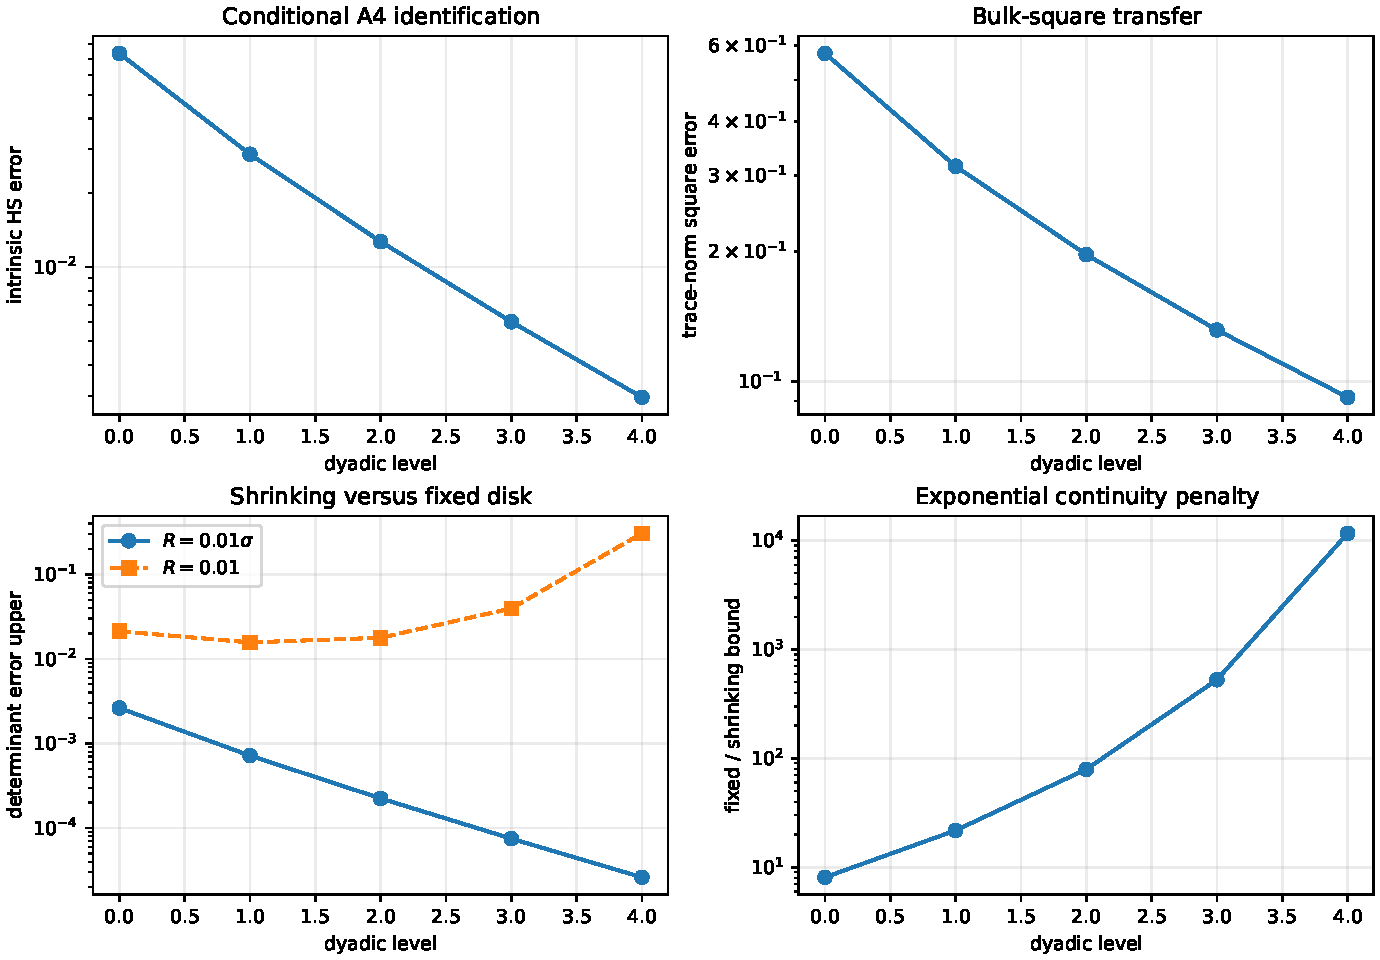
\includegraphics[width=0.98\textwidth]{figures/intrinsic_determinant_diagonal_transfer.pdf}
\caption{Conditional intrinsic error, square trace-norm transfer, shrinking
versus fixed determinant disks, and the exponential penalty ratio.}
\label{fig:audit}
\end{figure}

\section{Route consequence}

The Stage-A output is now sufficient for trace-class bulk squares along the
small-noise diagonal.  It also matches RH-46's natural shrinking coordinate
$w=O(\sigma)$.  What it does not supply is a nontrivial fixed-disk limit.

Stage A5 must therefore alter the object before taking the limit.  The two
remaining candidates are:
\begin{enumerate}[leftmargin=2.2em]
 \item divide out the explicit deterministic double-pole factor and prove a
       pole-renormalized determinant family is locally bounded;
 \item construct a relative determinant whose continuity depends on a
       renormalized trace norm rather than $\norm{B_\sigma^2}_1=O(\sigma^{-1})$.
\end{enumerate}
RH-80 tests this entry gate.

This paper is conditional on an all-level RH-78 corridor.  It does not close
Stage A1, unconditional Stage A4, or Stage A5; construct a Hilbert--Polya
operator; prove a $T\log T$ law or prime-power trace formula; identify zeta
zeros; or prove the Riemann Hypothesis.

\section{Conclusion}

Intrinsic identification survives squaring and the strict diagonal limit.
Determinants also transfer, but only on the shrinking scale naturally selected
by the double-pole geometry.  The fixed-disk exponential barrier makes the next
move unambiguous: renormalize first, then seek a limit.

\bibliographystyle{plainnat}
\bibliography{references}
\end{document}
